% ---------- chapters/methodology.tex ----------
\chapter{Methodology}\label{ch:methodology}

\section{Architecture Overview}

\begin{figure}[!ht]
    \centering
    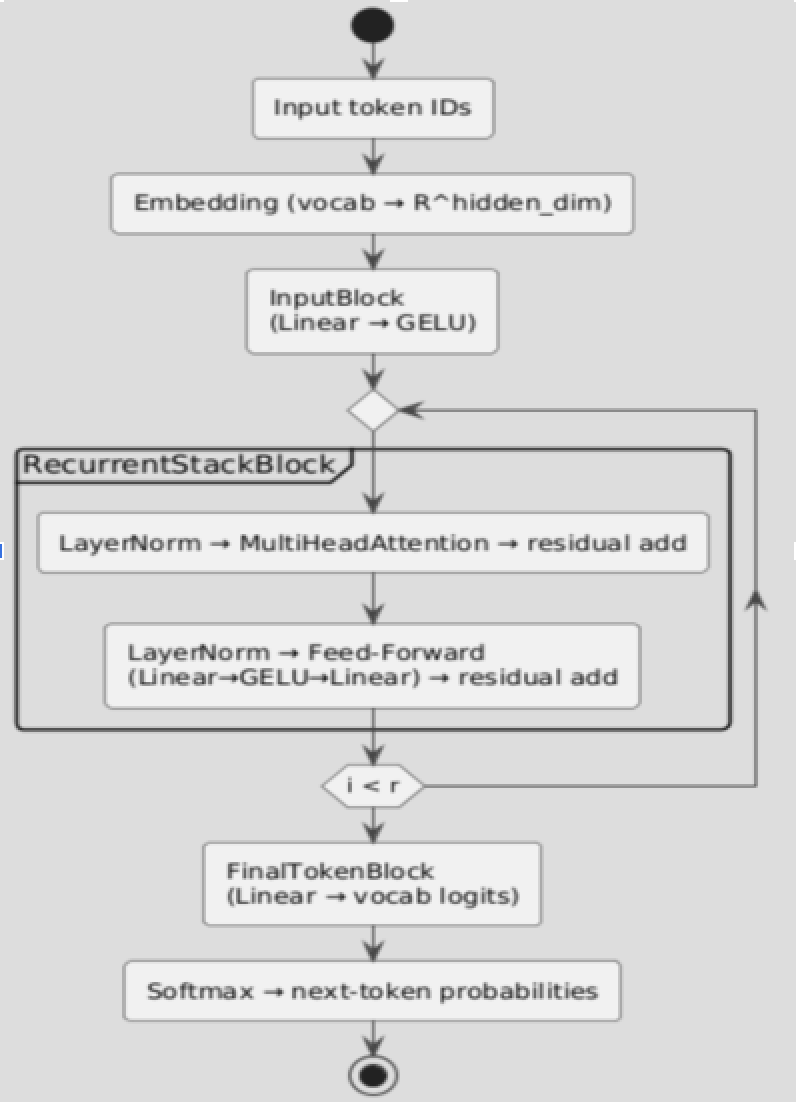
\includegraphics[width=0.4\textwidth]{figs/model_architecture.png}
    \caption{Data‑flow diagram of \texttt{ModularTextModel}.}
    \label{fig:model_arch}
\end{figure}

\texttt{ModularTextModel} (see \texttt{model.py}) is built from three
stacked modules:

\begin{enumerate}
    \item \textbf{Embedding \& Input projection} – token indices
          $\rightarrow$ hidden size $h=360$ via
          \texttt{nn.Embedding} followed by Linear+GELU.
    \item \textbf{Transformer Core} – 4layers, 12‑head attention,
          feed‑forward multiplier 4; this block can be repeated.
    \item \textbf{Output layer} – Linear map to vocabulary logits;
          only the last token’s logits are returned.
\end{enumerate}

Parameter count is roughly 60M, verified with
\texttt{random\_utils.py count\_params}.



\section{Recurrence in Practice}

The core loop is controlled by the argument
\texttt{num\_recurrences}.  
During evaluation we sweep
$r\in\{1,2,4,6,8,12,24\}$ to study depth–loss trade‑offs.
No token‑level replay or early‑exit logic is implemented in the current
codebase.

\section{Training Configuration}

\begin{itemize}
    \item \textbf{Dataset} – Hugging Face
          \texttt{nampdn-ai/tiny-strange-textbooks} (≈1M tokens),
          streamed line‑by‑line.
    \item \textbf{Sequence length} – 64 tokens produced with a sliding,
          left‑padded window.
    \item \textbf{Optimiser} – AdamW, learning‑rate $1\times10^{-3}$,
          batch 32.
    \item \textbf{Epochs} – default 3 (override with \texttt{-e} flag);
          one checkpoint per epoch in \texttt{./checkpoints/}.
\end{itemize}

\section{Evaluation Pipeline}

\begin{itemize}
    \item \texttt{main.py train} – launches training and saves
          checkpoints.
    \item \texttt{main.py manual} – interactive generation from a custom
          prompt.
    \item \texttt{main.py evaluate} – computes loss at each recurrence
          depth and writes CSV + plot to \texttt{./evaluation/}.
    \item \texttt{random\_utils.py} – helper for plotting
          \textit{training‑loss} and \textit{recurrence‑loss}.
\end{itemize}

Example commands:

\begin{verbatim}
# fresh training run (3 epochs, batch 32)
python main.py train -e 3 -b 32

# interactive generation using the latest checkpoint
python main.py manual

# sweep loss over recurrence depths
python main.py evaluate -r 1 2 4 6 8 12 24
\end{verbatim}
